\documentclass[sigconf,nonacm]{acmart}
\settopmatter{printacmref=false,printfolios=true}
\setcopyright{none}
\renewcommand\footnotetextcopyrightpermission[1]{}
\usepackage{amsmath,tabularx,array,enumitem}
\newcolumntype{Y}{>{\raggedright\arraybackslash}X}
\newcommand{\CourseNumber}{COMSCI/ECON 206}
\newcommand{\CourseName}{Computational Microeconomics}
\newcommand{\CourseSession}{Autumn 2026 Session 1}
\newcommand{\WorkshopSession}{[SESSION]}
\title{Who Pays to Know? Strategic Information Acquisition Before AI Collective Decisions}
\author{[AUTHOR NAME]}
\affiliation{\institution{Duke Kunshan University}\city{Kunshan}\country{China}}
\email{[EMAIL]}
\renewcommand{\shortauthors}{[AUTHOR NAME]}

\begin{document}
\begin{teaserfigure}
  \centering
  \IfFileExists{figures/ps1_teaser.pdf}{%
    \includegraphics[width=\textwidth]{figures/ps1_teaser.pdf}%
  }{%
    \IfFileExists{../figures/ps1_teaser.pdf}{%
      \includegraphics[width=\textwidth]{../figures/ps1_teaser.pdf}%
    }{%
      \fbox{\parbox[c][3.25in][c]{0.92\textwidth}{\centering
        Figure 1 vector PDF pending manual Draw.io export.}}%
    }%
  }
  \caption{Research design for costly information acquisition before a collective decision. Agents A and B independently choose Research or Skip. Each researcher pays private cost \(c\), while both agents receive information value \(V\) if at least one researches. The formal game creates free-riding incentives. Baseline equilibria and the discrete cost sweep were checked computationally with NashPy; tests of beliefs and bounded strategic reasoning remain planned.}
  \Description{A left-to-right formal-game mechanism begins with private research cost c and collective information value V. Agents A and B independently choose Research or Skip; a researcher pays c. If either researches, information is shared before a collective decision, leading to free-riding incentives and Nash equilibria. Below, economics connects private cost and shared benefit to equilibrium, computation connects payoff matrices and NashPy to a verified baseline and cost sweep, and behavior connects beliefs and bounded reasoning to a planned test. Solid connectors mark modeled or computationally checked relationships; a dashed connector marks the planned behavioral extension. Formal equilibria are computationally verified, while model-behavior comparison is not yet tested.}
  \label{fig:teaser}
\end{teaserfigure}
\maketitle
\noindent\textbf{Submission to:} \CourseNumber{} --- \CourseName.
\textbf{Course session:} \CourseSession.
\textbf{Workshop:} \WorkshopSession.
\textbf{NetID:} [NETID].
\textbf{Instructor:} Luyao Zhang. \textbf{Assignment:} PS1 research proposal.

\section{Three Connected Research Questions}
Before a collective AI decision, one agent's research can benefit both agents, although the researcher alone pays its cost. This creates a free-riding problem for AI-system designers and people relying on collective recommendations. Persico's committee model likewise studies costly information gathering before a group decision, with information as a public good; its voting environment differs from ours~\cite{persico2004}. Figure~\ref{fig:teaser} separates the completed formal benchmark from a future behavioral test.

\noindent\textbf{Q1---Economics:} How do private research costs shape strategic information acquisition and free-riding before a collective AI decision?
\textbf{Q2---Computation:} Can reproducible game-theoretic computation recover the predicted equilibria and show how equilibrium behavior changes as research costs vary?
\textbf{Q3---Behavior:} Do decision-makers follow equilibrium free-riding incentives, or can bounded reasoning and beliefs about others' willingness to research produce departures?
\textbf{Integrated:} When information is costly but collectively valuable, when will AI agents research rather than free-ride, and how closely will observed behavior match the formal prediction?
Economics supplies the incentive benchmark; computation makes it reproducible; behavior tests whether actual choices conform. The final comparison remains unanswered.

\section{Answer to Q1: Incentives and Intellectual Lineage}
Agents A and B simultaneously choose Research (R) or Skip (S) before a collective decision. A pure strategy chooses one action; a mixed strategy assigns probabilities to both. If either researches, each gains information value \(V\), and each researcher pays private cost \(c\); otherwise both receive zero. One research action supplies the full value. The baseline assumes common knowledge of \(V\), \(c\), actions, and payoff structure. We use Nash equilibrium~\cite{nash1950}.

For \(V=4,c=2\), payoffs are ordered (A,B):
\begin{center}
\begin{tabular}{c|cc}
 & B:R & B:S\\\hline
A:R & (2,2) & (2,4)\\
A:S & (4,2) & (0,0)
\end{tabular}
\end{center}
When the other researches, Skip saves \(c\) while preserving \(V\). When the other skips and \(0<c<V\), Research yields \(V-c>0\). Thus the author's initial theoretical predictions, (R,S) and (S,R), are pure equilibria; both were later verified independently and with NashPy. A third, symmetric mixed equilibrium has each player research with probability \(0.5\), also verified. Persico~\cite{persico2004} supplies a related costly-information incentive question, not this game's payoffs or AI evidence.

\section{Answer to Q2: Method and Evaluation}
Python constructs the \(V,c\) payoff matrices. Direct enumeration checks all four pure profiles; NashPy support enumeration cross-checks them and finds the interior mixed profile. At \(V=4,c=2\), both pure methods agree, and NashPy gives \([0.5,0.5]\) for each player in [R,S] order. Holding \(V=4\), tested interior costs \(c=1,2,3\) yield mixed Research probabilities \(0.75,0.50,0.25\). These match the analytical \(p(R)=1-c/V\) for \(0<c<V\). At \(c=4\), the equal-value boundary has pure (R,S), (S,R), and (S,S); at \(c=5\), only (S,S) is pure. Boundary support enumeration does not characterize every possible mixed profile.

The project preserves JSON/CSV outputs, an executed notebook, a public browser-based formal-model prototype, and a cost-sweep figure. All 24 current automated tests pass; a fresh notebook execution and independent project checks pass. Run the project-root verification script. These results concern equilibrium calculations, not empirical behavior.

\balance
\section{Answer to Q3: Behavior and Competing Explanations}
This answer is prospective. One explanation for future choices is strategic free-riding with correct beliefs about the other's choice; another is bounded strategic reasoning or inaccurate beliefs. Cognitive hierarchy models motivate the latter possibility~\cite{camerer2004}; research on higher-order beliefs in LLMs motivates testing it in AI settings~\cite{zhang2025}. Neither mechanism was estimated here.

A next study would hold payoffs fixed, elicit or manipulate beliefs about the other's Research choice, observe Research/Skip choices, and compare them with formal best responses. Choice and elicited belief data could distinguish predictions, though they would not directly reveal internal cognition. No real AI or human behavioral data are reported in PS1.

\section{Advanced Development and Future Directions}
The enduring question is who pays to become informed when information benefits a group. Nobel-recognized information economics highlights the importance of information and incentives~\cite{nobel2001stiglitz}; Persico gives a closer committee-acquisition foundation~\cite{persico2004}. The 1975 Turing Award to Newell and Simon marks a broad AI and cognition lineage~\cite{acm1975newellsimon}. Today, AI agents may participate in collective decisions, but this project's behavioral question remains open.

\noindent\textbf{Current research contribution:} The current contribution is a formal and reproducible baseline for studying costly information acquisition before collective AI decisions, together with a clearly testable behavioral gap.

\noindent\textbf{Roadmap:} Foundation: information incentives and computational cognition. PS1: a formal game, verified computation, and an interactive static educational prototype. Next: actual AI or human choice and belief study. Longer term: test mechanisms that assign research responsibility efficiently and robustly; none is developed here.

\noindent\textbf{Expected 2056 Nobel Prize and Turing Award contribution statement.}
By 2056, I aspire to develop and test economic and computational designs for assigning the cost of becoming informed in AI-assisted group decisions, integrating incentive theory, reproducible computation, and behavioral evidence. Milestones would include behavioral validation and mechanism evaluation; no award or impact is predicted.

\noindent\textbf{Open Science Statement.}
The \href{https://github.com/micL1222/PS1-Yiqiao/tree/v2-information-acquisition}{public GitHub v2 branch} contains code, notebook, outputs, tests, demo, and paper source. The \href{https://colab.research.google.com/github/micL1222/PS1-Yiqiao/blob/v2-information-acquisition/notebooks/information_acquisition_baseline.ipynb}{Google Colab notebook} fetches that branch. Verified computational/artifact snapshot: \href{https://github.com/micL1222/PS1-Yiqiao/commit/b986771d1e79979825cd375c8ed663994bdc67ec}{\texttt{b986771}}.

Run \texttt{./scripts/verify\_all.sh} locally. No explicit reuse license has yet been granted; public availability should not be interpreted as additional reuse permission.

\noindent\textbf{Statement of Contribution to the UN's SDGs.}
The released \href{https://huggingface.co/spaces/dku-comsci-econ206-2026/who-pays-to-know}{Hugging Face Static Space} is an interactive educational prototype: students can vary \(V,c\) and observe changes in payoff matrices, best responses, pure Nash equilibria, the mixed-strategy benchmark, and free-riding incentives. This possible use aligns with SDG 4's quality-education aim~\cite{un_sdg4}. A future pre/post equilibrium-identification task could assess learning. Educational effectiveness has not been evaluated.
\label{main:end}


\clearpage
\section*{Author Notes}
\subsection*{Acknowledgements}
The author acknowledges Prof. Luyao Zhang, Program Chair, and Prof. Ken Rogerson, Program Discussant, of the 2056 Nobel and Turing Laureate Program Launch Workshop at Duke Kunshan University on September 7, 2026. Workshop session: [WORKSHOP SESSION]. Assigned role: [ROLE]. Teammates: [TEAMMATE 1], [TEAMMATE 2]. Specific contributions and class acknowledgements: [AUTHOR TO VERIFY AND COMPLETE].
\subsection*{Individual Contribution}
The author developed the revised research problem and strategic direction, specified and interpreted the model, and retains responsibility for all final claims. OpenAI Codex assisted with implementation, debugging, tests, notebook and artifact organization, local demo development, drafting assistance, citation checking, and consistency verification. Codex is not a coauthor. Human verification of this draft is pending.

\bibliographystyle{ACM-Reference-Format}
\bibliography{references}
\clearpage\onecolumn
\appendix
\section{Technical Details and Reproducibility}
\label{app:technical}
For each agent \(i\), \(u_i=V\mathbf{1}\{a_A=R\ \mathrm{or}\ a_B=R\}-c\mathbf{1}\{a_i=R\}\), with \(V>0,c\geq0\). A and B choose simultaneously; the action order in code is [Research, Skip]. One research action is sufficient for the full information value. For \(V=4,c=2\), the matrices are \(A=\left[\begin{smallmatrix}2&2\\4&0\end{smallmatrix}\right]\) and \(B=\left[\begin{smallmatrix}2&4\\2&0\end{smallmatrix}\right]\). Direct best-response enumeration tests all four pure action profiles, including ties; NashPy support enumeration provides a separate computation.

Let \(p\) be the probability that the \emph{other} player researches. Research yields \(U(R)=V-c\), while Skip yields \(U(S)=pV\). Interior indifference requires \(V-c=pV\), hence \(p=1-c/V\) for \(0<c<V\). The formula predicts \(0.75,0.50,0.25\) for \(c=1,2,3\) at \(V=4\), exactly matching the tested NashPy profiles. At \(c=0\), pure equilibria are (R,R), (R,S), (S,R). At \(c=4\), they are (R,S), (S,R), (S,S); at \(c=5\), only (S,S) is pure. The two boundary cases are degenerate, and finite support output is not a full account of boundary mixed-equilibrium continua. Invalid \(V\leq0\) and \(c<0\) are rejected by tests.

The source is \url{src/information_acquisition_game.py}; the runner is \url{src/run_baseline_analysis.py}. Saved evidence is \url{outputs/baseline_equilibria.json}, \url{outputs/cost_sweep.csv}, \url{outputs/verification_summary.md}, and \url{notebooks/information_acquisition_baseline.ipynb}. The original suite has 14 model tests and 10 demo-logic tests. A fresh notebook run executes six code cells; the project validator passes 16 checks. The local demo uses the same model and illustrates formal choices, not observed decisions.

The tested computational environment was Python 3.9.6, NumPy 2.0.2, NashPy 0.0.41, pandas 2.3.3, and matplotlib 3.9.4. The demo environment was Python 3.9.6 with Gradio 4.44.1. Dependencies in the repository are unpinned; these are the recorded tested versions, not a promise of identical behavior in every future environment. No stochastic seed is relevant to these deterministic checks. The cost-sweep vector figure below is generated from the saved CSV. It shows equilibrium probabilities, not observed Research frequencies.

\begin{figure}[h]
\centering
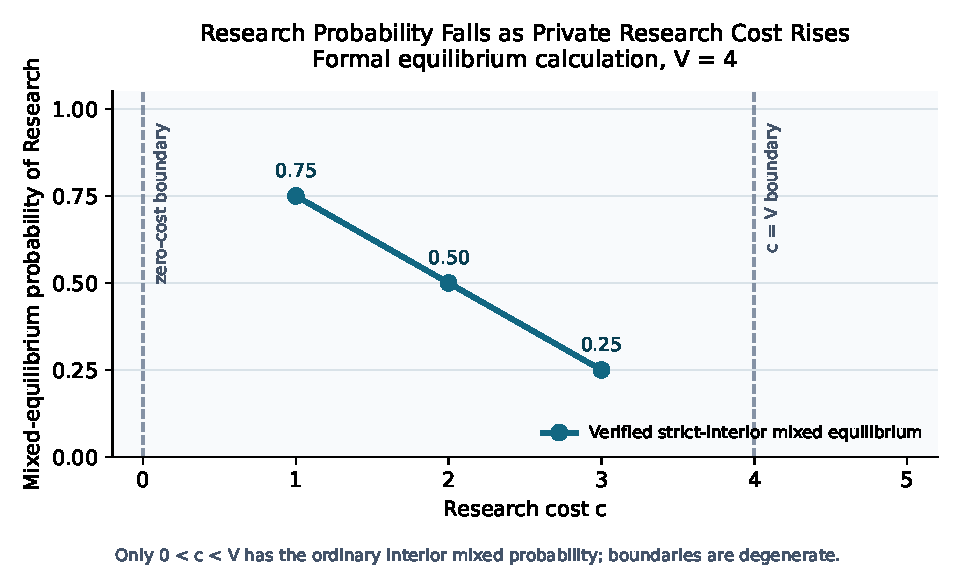
\includegraphics[width=0.65\textwidth]{figures/cost_sweep_mixed_probability.pdf}
\caption{Formal mixed-equilibrium Research probability at \(V=4\) for tested strict-interior costs \(c=1,2,3\). These are theoretical equilibrium probabilities confirmed by computation, not empirical frequencies. Boundary cases are handled separately.}
\Description{Three plotted points decrease from 0.75 at cost 1, to 0.50 at cost 2, to 0.25 at cost 3. They are computed formal equilibrium probabilities.}
\end{figure}

No real LLM or human choices, learning outcomes, or causal mechanism effects were measured.

\subsection{AI-Use Disclosure}
\label{app:ai}
On 2026-09-20, OpenAI Codex assisted after the author's initial independent reasoning with project initialization, implementation, debugging, tests, notebook construction, artifact construction, local demo development, LaTeX drafting, citation checking, and consistency validation. The research direction, substantive choices, interpretation, and final responsibility belong to the author. The project-level \texttt{AI\_USE\_LOG.md} records the stages. Suggestions and draft claims remain subject to author review; human verification has not been marked complete. Initial reasoning, handwritten reflection, and peer reviews are Human-Only. No peer-review file was accessed for this draft.

\section{Cumulative Intellectual Development}
\label{app:development}
The earlier v1 project studied AI attention, interruptions, and reputation-calibrated scheduling. Multiple agents submitted information, but an attention coordinator chiefly scored and scheduled their interruptions. The author concluded that direct strategic interdependence between two decision makers was not sufficiently central or explicit: one agent's optimal action was not clearly contingent on another agent's action, and players, actions, payoffs, best responses, and equilibrium were not the organizing model. This was the author's own reassessment, not a change attributed to either peer review.

The author therefore selected costly information acquisition before a collective AI decision. Two agents directly choose Research or Skip. If the other researches, Skip preserves the shared information benefit without paying the private cost; if the other skips and \(0<c<V\), Research is individually worthwhile. The resulting best responses depend on the opponent's action, making free-riding and equilibrium central. Economics explains the incentives, computation makes the benchmark reproducible through payoff matrices, independent checks, NashPy, a cost sweep, a notebook, tests, and a local prototype, and behavioral science asks whether future observed choices follow that benchmark or differ with beliefs and bounded reasoning. These lenses address one mechanism. The small baseline also permits analytical predictions, computational checks, and explicit separation from future behavioral evidence. Asymmetric costs, signal quality, repeated interaction, larger groups, aggregation, and responsibility mechanisms remain future extensions, not implemented results.

Within the revised game, the author initially predicted the two pure equilibria \((R,S)\) and \((S,R)\). NashPy verified them and additionally identified a symmetric mixed equilibrium. A subsequent indifference calculation yielded \(p(\text{Research})=1-c/V\) for the strict interior \(0<c<V\), agreeing with the tested interior costs. Computation thus revealed equilibrium structure beyond the author's initial pure-strategy reasoning, which was then analytically checked.

The 2056 Nobel and Turing Laureate Program Launch Workshop took place September 7, 2026 at Duke Kunshan University, IB 2050; Prof. Luyao Zhang was Program Chair and Prof. Ken Rogerson was Program Discussant. The author's earlier workshop session was Session B. No workshop comment or peer-review claim is inferred or attributed here. Any course-required handwritten reflection remains the author's own Human-Only work.

\section{Field Trip and Open-Source Inspiration}
\label{app:field}
The author confirms attending both the Tencent Shanghai Office and Shanghai Science and Technology Museum on September 4, 2026 and personally taking both photographs. The files were copied unchanged from the author's v1 project. The images record visible displays, not evidence for the present game's equilibria or observed free-riding.

\subsection{Tencent Shanghai Office --- September 4, 2026}
\begin{center}
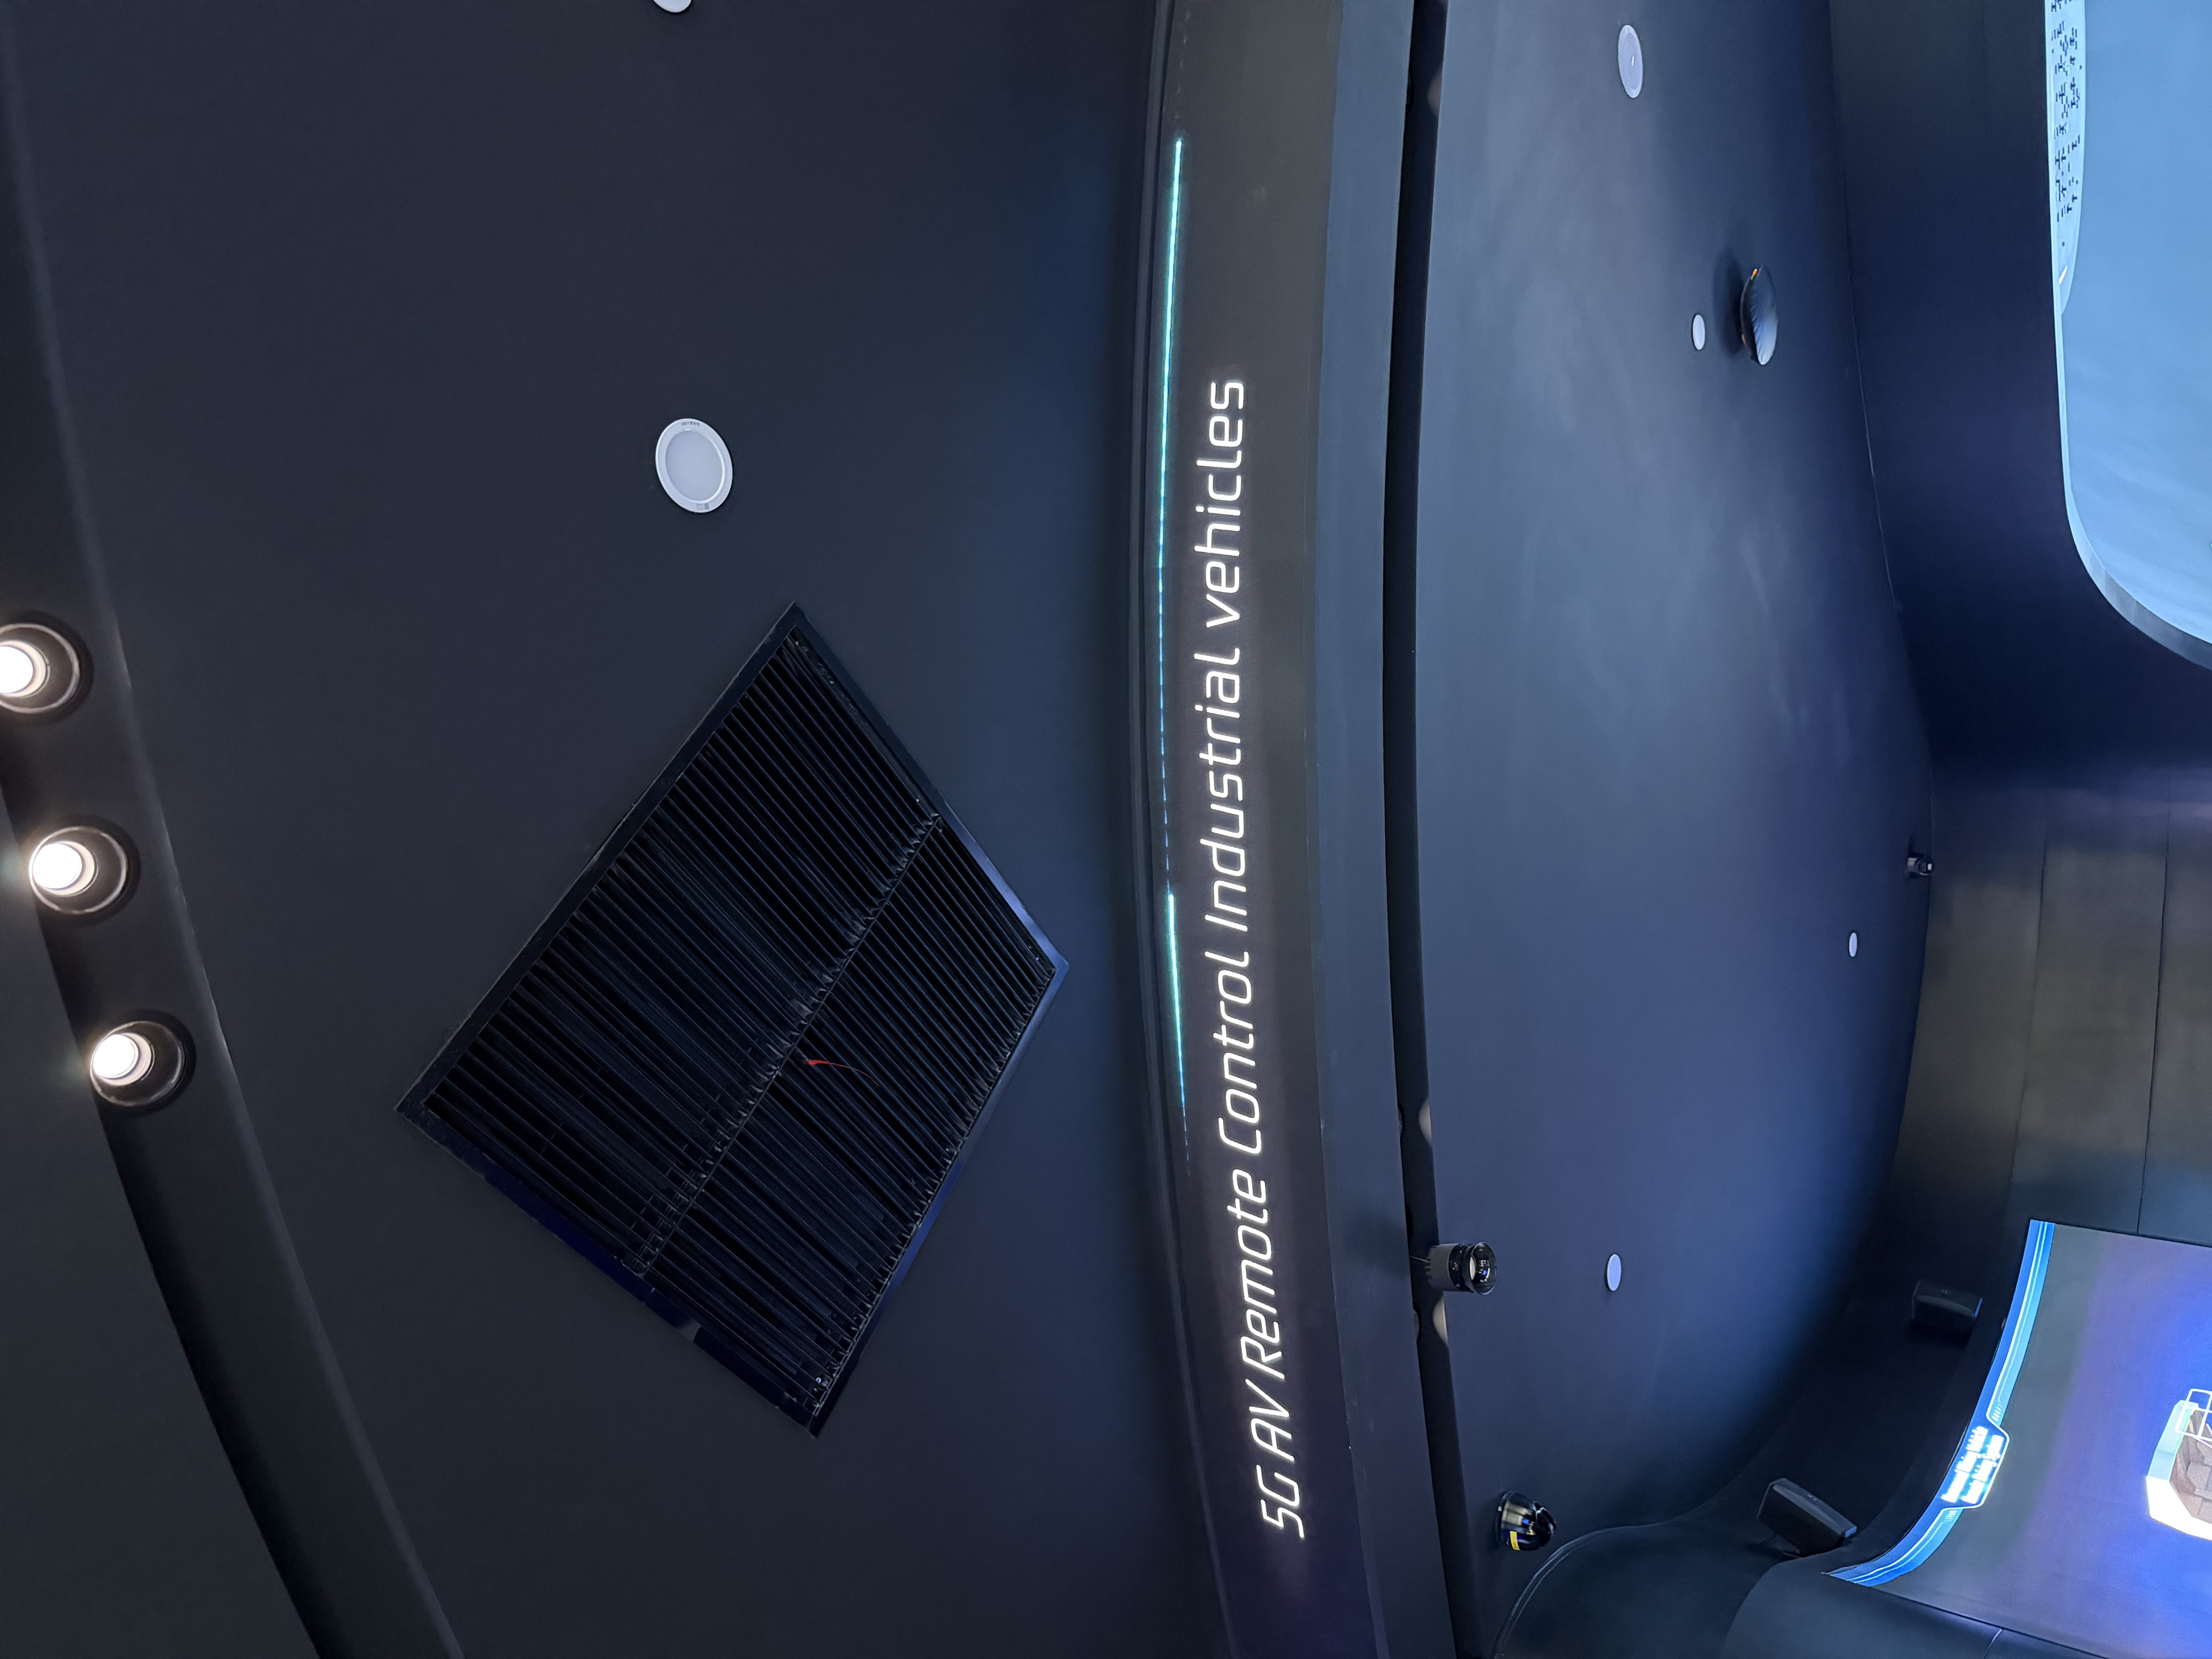
\includegraphics[width=0.55\linewidth,angle=-90]{field_trip/tencent_shanghai_office.jpg}
\end{center}
\noindent\textbf{Photograph caption:} Technology display at Tencent Shanghai Office with the visible heading ``5G AV Remote Control Industrial Vehicles.'' Photograph by Yiqiao Liu (Mickey), September 4, 2026.

\noindent\textbf{Observation:} The photograph shows an illuminated heading and part of a technology display. \textbf{Interpretation:} The visit exposed the author to practical automated systems and motivated broader questions about coordination and responsibility; the image does not show strategic information acquisition or a tested equilibrium.

\subsection{Shanghai Science and Technology Museum --- September 4, 2026}
\begin{center}
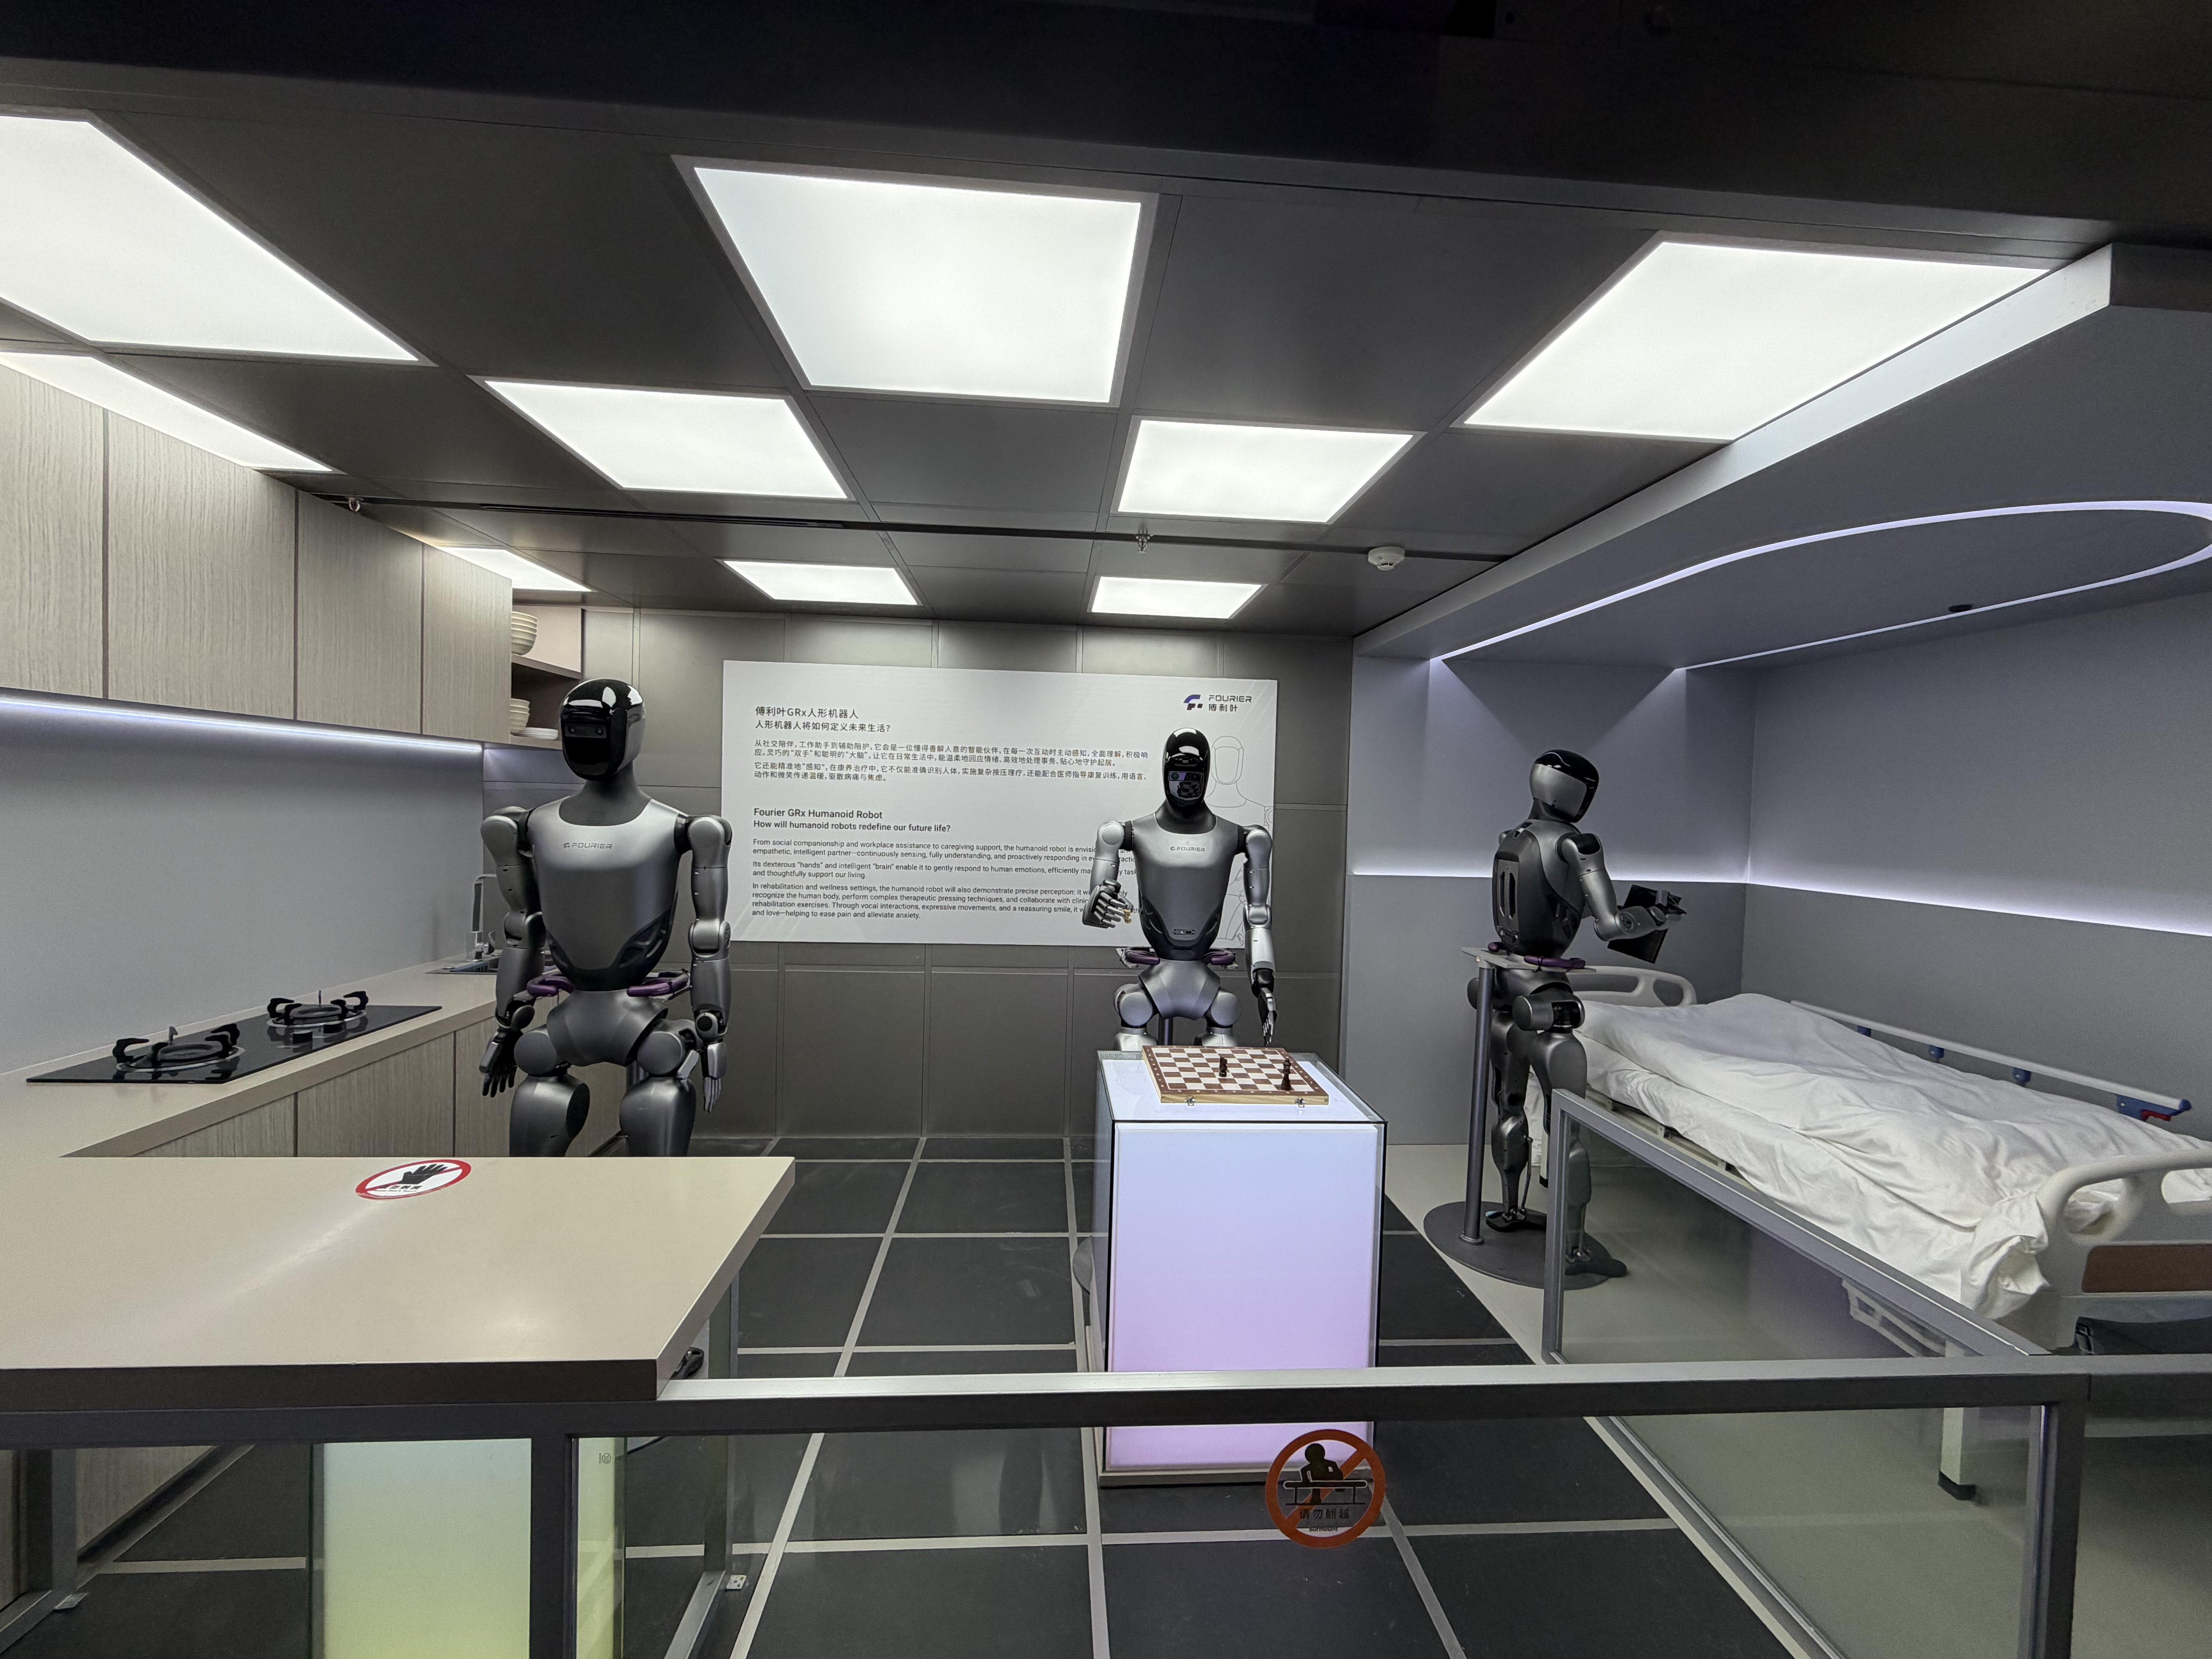
\includegraphics[width=0.62\linewidth]{field_trip/shanghai_science_technology_museum.jpg}
\end{center}
\noindent\textbf{Photograph caption:} Humanoid-robot exhibit at Shanghai Science and Technology Museum. Photograph by Yiqiao Liu (Mickey), September 4, 2026.

\noindent\textbf{Observation:} The photograph shows humanoid-robot figures, an exhibit panel, a chessboard, and a bed in a staged room. \textbf{Interpretation:} The exhibit prompted broader questions about how automated systems may coordinate decisions and responsibilities. It does not demonstrate free-riding, Nash equilibrium, or the current model's behavior.

\section{Historical Review and Revision Record}
\label{app:review}
\subsection{Review-process status}
The original PS1 v1 studied AI attention and interruption scheduling. One accessible peer review concerns that earlier topic. It is retained as historical review-process evidence, not treated as direct evaluation of the v2 information-acquisition model. One assigned peer review is currently inaccessible to the author. Its substantive content has not been incorporated into this v2 revision. Neither review's substantive contents are quoted, summarized, or inferred here.

\subsection{Major revision decision}
The topic change was the author's own research decision and is not attributed to either reviewer. Although v1 included multiple agents, they mainly submitted information to an attention coordinator. Direct strategic interdependence between two decision makers was not sufficiently central or explicit: one player's best action was not cleanly defined by the other's action. In v2, two players choose Research or Skip, their payoffs depend on both choices, and best responses and equilibrium organize the economics, reproducible computation, and a future behavioral comparison.

\subsection{Objective v1-to-v2 revision record}
\begin{table}[H]
\caption{Objective development record; no reviewer-specific cause is inferred.}
\begin{tabularx}{\textwidth}{@{}p{0.16\textwidth}p{0.19\textwidth}p{0.19\textwidth}p{0.22\textwidth}Y@{}}
\toprule
Earlier state & Revision & Reason & Evidence / verification & Affected artifact\\\midrule
Attention/interruption scheduling & Costly information-acquisition game & Make direct strategic interdependence central & Current formal model & Research model, paper\\
Agents mainly submitted to a coordinator & Two players directly choose Research or Skip & Make each best response depend on the other player's action & Payoff matrices and independent best-response analysis & \texttt{src/}, \texttt{tests/}\\
Economics was not sufficiently central to scheduling & Private cost and shared benefit create free-riding & Make incentives and equilibrium core & Verified Nash equilibria & Model, outputs\\
Two pure equilibria initially predicted for v2 & NashPy identified an additional mixed equilibrium & Check the full baseline equilibrium structure & \texttt{baseline\_equilibria.json} and analytical cross-check & Notebook, outputs\\
No current-topic interactive artifact & Public Static Space & Make the formal game inspectable & Live app and Python--JavaScript parity & \texttt{deployment/}\\
\bottomrule
\end{tabularx}
\end{table}

\subsection{Response status}
One accessible review evaluates the superseded v1 topic and is retained as historical review-process evidence. Another assigned review is currently inaccessible to the author; therefore no substantive response to unavailable content is claimed. Any course-required Human-Only response remains to be completed by the author if the material becomes available or the instructor gives alternative instructions.

\section{Structured Abstract and Cumulative Proposal Map}
\label{app:abstract}
\begin{table}[H]
\caption{Eight-row structured abstract; actual results and future work remain distinct.}
\begin{tabularx}{\textwidth}{@{}p{0.28\textwidth}Y@{}}
\toprule
Proposal element & Current statement / change\\\midrule
Background & Collective decisions may benefit from information acquired privately before action; costly acquisition creates a public-good incentive question.\\
Motivation and application & In an AI-assisted group decision, agents or designers must decide who bears research cost when all benefit. Users of collective recommendations are stakeholders.\\
Three connected questions & Economics asks how cost affects free-riding; computation asks whether equilibria and cost changes are reproducible; behavior asks whether choices reflect strategic incentives or bounded beliefs. Together: when will agents acquire information, and will observed choices match the benchmark?\\
Method and model assumptions & Two agents simultaneously choose Research or Skip; one Research supplies value \(V\) to both and each researcher pays \(c\). Baseline \(V=4,c=2\), common knowledge, Nash equilibrium, NashPy plus independent best responses.\\
Results or expected results & \textbf{Actual:} two pure equilibria, symmetric \(p(R)=0.5\) mixed equilibrium, verified interior sweep \(0.75,0.50,0.25\), passing tests, executed notebook, and public Static Space. \textbf{Planned:} AI or human behavioral tests of choices and beliefs; no behavioral result exists.\\
Intellectual merits & The reproducible game clarifies a cost-sharing mechanism and specifies a behavioral gap that incentive theory alone cannot settle. Economics, computation, and behavior play distinct roles.\\
Practical impacts & \textbf{Existing:} a public interactive prototype for inspecting payoffs and equilibria. \textbf{Potential:} after validation, research-responsibility designs could inform organizational and public decisions. \textbf{Not evaluated:} improved learning or institutional efficiency. A pre/post best-response task could test the SDG 4 learning aim.\\
Feedback received and revision made & V1 focused on attention/interruption scheduling. The author reassessed its insufficiently explicit strategic interdependence and rebuilt v2 around costly information acquisition, aligning economics, computation, and behavior around one mechanism. One accessible review concerns v1; another assigned review is currently inaccessible. Neither is treated as direct v2 evidence.\\
\bottomrule
\end{tabularx}
\end{table}

\end{document}
